\documentclass{standalone}
\usepackage{tikz}
\usepackage{tikzscale}
\usetikzlibrary{arrows}
\usetikzlibrary{arrows.meta}
\usetikzlibrary{patterns}
\usetikzlibrary{shapes}
\usetikzlibrary{calc}
\usetikzlibrary{matrix}
\usetikzlibrary{positioning}
\usepackage{calc}
\usetikzlibrary{calc,trees,positioning,arrows,fit,shapes}

\usepackage{tkz-euclide}
\usetikzlibrary{
	angles,
	quotes,
}
\usepackage{pgfplots}

\begin{document}
	

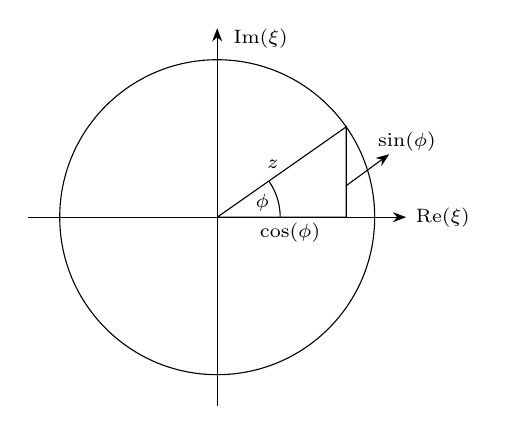
\begin{tikzpicture}
    [   baseline={([yshift=-5ex]current bounding box.north)}
    ,   > = Stealth
    ]
    ]
    \draw (0mm,0mm) circle (20mm);
    \draw[->] (-24mm,0mm) -- (24mm,0mm);
    \draw[->] (0mm,-24mm) -- (0mm,24mm);
    \coordinate (Z) at (35:20mm);

    \node[anchor = north west, inner sep = 0pt] at (2mm,24mm)
    {\scriptsize Im$(\xi)$};
    \node[anchor = west] at (24mm,0mm) {\scriptsize Re$(\xi)$};

    \draw[domain=0:35, smooth] plot ({8mm*cos(\x)},{8mm*sin(\x)});
    \node at (17.5:6mm) {\scriptsize$\phi$};

    \draw
    (0mm,0mm)
    -- node[anchor = north, inner sep = 2pt] {\scriptsize\hspace*{2ex}cos$(\phi)$}
    ({20mm*cos(35)},0mm)
    --
    (Z)
    -- node[anchor = south east, inner sep = 1pt] {\scriptsize$z$}
    (0mm,0mm);

    \node[anchor = south west, inner sep = 1pt] (S) at (20mm,8mm) {\scriptsize sin$(\phi)$};
    \draw[->] ({20mm*cos(35)},4mm) -- (S);
\end{tikzpicture}


\end{document}